% ----------------------- TODO ---------------------------
% Diese Daten müssen pro Blatt angepasst werden:
\newcommand{\NUMBER}{2}
\newcommand{\EXERCISES}{2}
\newcommand{\AUFGABENSTART}{1}
\newcommand{\DEADLINE}{Wednesday, 01-05-2024, 15:59}
% Diese Daten müssen einmalig pro Vorlesung angepasst werden:
\newcommand{\COURSE}{Software Engineering}
\newcommand{\TUTOR}{}
\newcommand{\STUDENTA}{Albert Ratschinski (5154309)}
\newcommand{\STUDENTB}{Severin Plewe (5333060)}
% ----------------------- TODO ---------------------------

\documentclass[a4paper]{scrartcl}

\usepackage[utf8]{inputenc}
\usepackage[ngerman]{babel}
\usepackage{dsfont}
\usepackage{amsmath}
\usepackage{amssymb} % Added for square symbols
\usepackage{fancyhdr}
\usepackage{color}
\usepackage{graphicx}
\usepackage{lastpage}
\usepackage{listings}
\usepackage{tikz}
\usepackage{pdflscape}
\usepackage{subfigure}
\usepackage{float}
\usepackage{polynom}
\usepackage{hyperref}
\usepackage{tabularx}
\usepackage{forloop}
\usepackage{geometry}
\usepackage{fancybox}
\usepackage{stmaryrd}
\usepackage{bbold}
\usepackage{xcolor}

\usetikzlibrary{calc,arrows}
\usepackage{listings}
\lstset{
    basicstyle=\small\ttfamily,
    breaklines=true,
    numbers=left,
    numberstyle=\tiny,
    frame=tb,
    columns=fullflexible
}

%Größe der Ränder setzen
\geometry{a4paper,left=3cm, right=3cm, top=3cm, bottom=3cm}

%Kopf- und Fußzeile
\pagestyle {fancy}
\fancyhead[L]{Tutor: \TUTOR}
\fancyhead[C]{\COURSE}
\fancyhead[R]{\today}

\fancyfoot[L]{}
\fancyfoot[C]{}
\fancyfoot[R]{Seite \thepage /\pageref*{LastPage}}

\newcounter{aufgabe}

%Formatierung der Überschrift, hier nichts ändern
\def\header#1#2{
  \begin{center}
    {\Large Exercise Sheet #1}\\
    {(Deadline #2)}
  \end{center}
}

\newcommand{\nextAufgabe}{
  \section*{Aufgabe \theaufgabe}
  \stepcounter{aufgabe}
}
\newcommand{\circled}[2]{
  \tikz[baseline=(char.base)]{
  \node[shape=circle,draw,color=#2,inner sep=2pt] (char) {#1};}
}

\newcommand{\rc}[1]{
  \circled{#1}{red}
}
\newcommand{\gc}[1]{
  \circled{#1}{green}
}
\newcommand{\bc}[1]{
  \circled{#1}{blue}
}

\newcommand{\R}{
  \mathbb{R}
}
\newcommand{\N}{
  \mathbb{N}
}
\newcommand{\Z}{
  \mathbb{Z}
}
\newcommand{\Q}{
  \mathbb{Q}
}
\newcommand{\C}{
  \mathbb{C}
}

\newcounter{spalte}
\newcounter{zeile}

\newcommand{\spalte}[3]{
\left(\begin{array}{c}
  #1   \\
  #2   \\
  #3   \\
\end{array}\right)
}
\newcommand{\spaltef}[4]{
\left(\begin{array}{c}
  #1   \\
  #2   \\
  #3   \\
  #4   \\
\end{array}\right)
}
\newcommand{\kopf}[4]{
  
    idx & 
    %x werte
      \setsepchar{ }
      \forloop{spalte}{0}{\value{spalte} < #1}%
        {
        \readlist\arg{#3}
        \arg[\fpeval{\thespalte+1}] &
        } 
      %funktionen
      \setsepchar{ }
      \forloop{spalte}{0}{\value{spalte} < #2}%
        {
        \readlist\arg{#4}
        \arg[\fpeval{\thespalte+1}] \ifthenelse{\fpeval{#2-1}=\thespalte}{}{&}
        }
        \\\hline 
}

\begin{document}

\begin{tabularx}{\linewidth}{m{0.5 \linewidth} X}
  \begin{minipage}{\linewidth}
    \STUDENTA\\
    \STUDENTB\\
  \end{minipage} &
\end{tabularx}
\setcounter{aufgabe}{\AUFGABENSTART}%
\header{Nr. \NUMBER}{\DEADLINE}

% ----------------------- TODO ---------------------------

\begin{center}
  \begin{tabular}{|c|cc|cccc|}
    \hline
    Task      & 1.1         & 1.2        & 2.1       & 2.2       & 2.3     & 2.4  \\
    \hline
    Completed & $\boxtimes$ & $\boxtimes$  & $\boxtimes$ & $\boxtimes$ & $\boxtimes$ & $\boxtimes$ \\
    \hline
    Feedback  & \textcolor{red}{$\boxtimes$} & $\square$    & $\boxtimes$ & $\square$ & $\square$ & $\boxtimes$ \\
    \hline
  \end{tabular}
\end{center}
\begin{center}
  \textbf{Question: Are we allowed to take in a 3-rd person in our group?}
\end{center}

\section*{Exercise 1 -  Cyclomatic Complexity}

\subsection*{Exercise 1.1}

\begin{figure}[h]
  \centering
  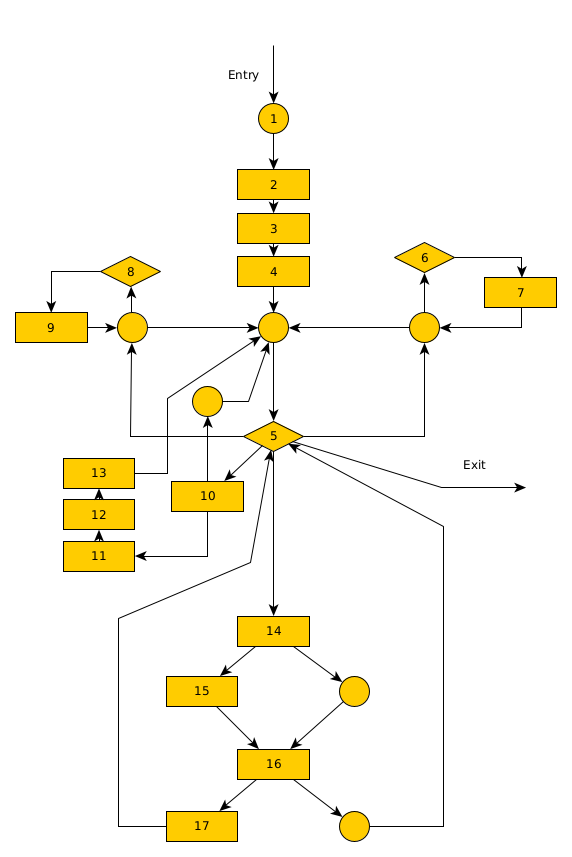
\includegraphics[width=0.5\textwidth]{cyclomaticComplexity.png}
  \caption{Control Flow Graph for \textit{qucikSort()}}
\end{figure}

To calculate the cyclomatic complexity of the given control flow graph we can use the formula:
\begin{center}
  $v(G) = |E| - |V| + p$
\end{center}

We yeild:
\begin{center}
  Number of nodes: 23 \\
  Number of edges: 31 \\
  $V(G) = 31 - 23 + 2 = 6$
\end{center}

\subsection*{Exercise 1.2}
The alternative choice of the CFG construction would not alter the value of the cyclomatic Complexity metric since:
\begin{center}
  $V(G) = |E| - |V| + p = 10 - 9 + 2 = 3$
\end{center}
which is the holds the same value as the original CFG. We can thereby conclude that the cyclomatic complexity metric 
is independent of wheather we chose one version or the other. For overview sake I would argue that represented version 
is way more readable and easier to understand.

\section*{Exercise 2 - Cost Estimation}
\subsection*{Exercise 2.1}
\textbf{Estimation of Overall Development Effort in Person-Months (PM)}

\begin{enumerate}
    \item \textbf{Definition of Person-Month:} A person-month represents the amount of work one person can complete in one month. It's calculated by multiplying the number of people working on a project by the number of months they work.
    
    \item \textbf{Calculation:}
    \begin{itemize}
        \item Each team member contributes approximately 180 hours of work.
        \item Assuming an average of 6.5 team members.
        \item Total hours contributed by the team per month: $6.5 \times 180 = 1170$ hours.
        \item Typical number of working hours in a month is assumed to be 160.
        \item Person-months $= \frac{1170 \text{ hours}}{160 \text{ hours}} \approx 7.3125 \text{ PM}$.
    \end{itemize}
    
    \item \textbf{Result:} The estimated overall development effort for this project is approximately 7.31 person-months.
\end{enumerate}
\textbf{Question from the student:} \textit{How would we calculate the PM from given information of the slide?}

Definition of [PM (person-months)] from the slides:
\begin{center}
  \textit{Person-months (PM) is a unit of measurement that
   represents the amount of work performed by a person in one month.} \\
  $E = a \cdot (\frac{S}{kDSI})^b$
\end{center}

Where:
\begin{itemize}
  \item $E$ is the effort in person-months
  \item $S$ is the size of the software product in DSI (Delivered Source Instructions)
  \item $a$ and $b$ are constants
  \item $k$ is a constant \textit{what does it stand for?}
\end{itemize}

\subsection*{Exercise 2.2}
We conducted a thorough analysis of the requirements specified in Appendix A for the development of the video game. Taking into consideration the multifaceted nature of the functional and quality requirements, as well as the additional constraints delineated, we have estimated the delivered KLOC (Thousand Lines of Code) to fall within the range of 50-70 KLOC.

\begin{itemize}
  \item Functional requirements complexity
  \item Quality requirements demands
  \item Additional constraints imposition
  \item Continuous code maintenance necessity
  \item Complexity of player interactions
  \item Real-time gameplay requirements
  \item Scalability and extensibility considerations
  \item Usability and user experience implementation
\end{itemize}

\subsection*{Exercise 2.3}

\begin{table}[h]
  \centering
  \begin{tabular}{|l|l|}
  \hline
  \textbf{Cost Driver} & \textbf{Rating} \\
  \hline
  \textbf{Product Attributes} &  \\
  \hline
  Required Software Reliability & High \\
  Size of Application Database & High \\
  Complexity of the Product & Nominal \\
  \hline
  \textbf{Hardware Attributes} &  \\
  \hline
  Run-time Performance Constraints & High \\
  Memory Constraints & Nominal \\
  Volatility of the Virtual Machine Environment & Nominal \\
  Computer Turnaround Time & Nominal \\
  \hline
  \textbf{Personnel Attributes} &  \\
  \hline
  Analyst Capability & Nominal \\
  Applications Experience & Nominal \\
  Software Engineer Capability & Nominal \\
  Virtual Machine Experience & Nominal \\
  Programming Language Experience & Nominal \\
  \hline
  \textbf{Project Attributes} &  \\
  \hline
  Use of Modern Programming Practices & Nominal \\
  Use of Software Tools & Nominal \\
  Required Development Schedule & Nominal \\
  \hline
  \end{tabular}
  \caption{Cost Drivers and Ratings}
  \label{tab:cost_drivers}
  \end{table}

  \begin{itemize}
    \item Required Development Schedule
    \textbf{Rating:} Nominal \\
    \textbf{Explanation:} The project's development schedule is expected to follow the nominal timeline, with minor flexibility but no significant deviations.
    
    \item Required Software Reliability
    \textbf{Rating:} High \\
    \textbf{Explanation:} Given the potential consequences of software failures in the game project, a high level of reliability is crucial to avoid significant financial losses or human inconveniences.
    
    \item Use of Modern Programming Practices
    \textbf{Rating:} Nominal \\
    \textbf{Explanation:} While the project aims to incorporate modern programming practices, such as structured design and incremental development, not all practices are fully leveraged, resulting in a nominal rating.
  \end{itemize}

\subsection*{Exercise 2.4}
\textbf{Calculation of Effort Adjustment Factor (EAF)}
\begin{align*}
  EAF &= \prod_{i=1}^{n} C_i \\
  &= 1.15 * 1.08 * 1.00 * 1.11 * 1.00 * 1.00 * 1.00 * 1.00 * 1.00 * 1.00 * 1.00 * 1.00 * 1.00 * 1.00 * 1.00 \\
  &= 1.3786
  \end{align*}

\textbf{Calculation of estimated effort in person-months (E)}
\begin{align*}
  E &= a * (KLOC)^b * EAF \\
  &= 3.2 * (50)^{1.05} * 1.3786 \\
  &=  268.2296 \\
\end{align*}
To break it down: 
\begin{itemize}
  \item Each team member contributes approximately 268 hours of work.
  \item Assuming an average of 6.5 team members.
  \item Total hours contributed by the team per month: $6.5 \times 268 = 1742$ hours.
  \item Typical number of working hours in a month is assumed to be 160.
  \item Person-months $= \frac{1742 \text{ hours}}{160 \text{ hours}} \approx 10.8875 \text{ PM}$.
  \item Therefore the difference between the estimated effort and the actual effort is $10.8875 - 7.3125 = 3.575$ PM.
\end{itemize}

\textbf{Reasons for the deviation in the estimated effort:}
\begin{itemize}
  \item Inaccurate Estimation of Cost Drivers: The ratings assigned to the cost drivers in the COCOMO calculation might not accurately reflect the true impact of these factors on the project's effort.
  \item The COCOMO calculation might have considered additional factors or complexities that were not fully accounted for in the initial estimation.
\end{itemize}

\end{document}
